\subsection{Traditional Quantitative Paraphrase Evaluation Measures}
\label{subsec:traditional_quantitative_evaluation_measures}

The evaluation of paraphrases can be broadly divided into syntactic and semantic approaches~\citep{gohsen_captions_2023}. 
Syntactic metrics primarily assess measure n-gram overlaps between a candidate text and reference texts~\citep{zhou_paraphrase_2021}. 
By contrast, semantic metrics aim to capture equivalence of meaning. 
Combining both perspectives allows identification of good paraphrases which balance syntactic diversity and semantic similarity.

% \citet{gohsen_captions_2023} normalized all metrics and averaged the semantic and syntactic scores separately.

\subsubsection{Syntactic Measures}
Syntactic evaluation metrics mainly focus on the n-gram overlaps~\citet{zhou_paraphrase_2021}. 
Common syntactic evaluation metrics include \acs{bleu}, \acs{rouge}-1, \acs{rouge}-L.

BLEU~\citep{papineni_bleu_2001} was originally developed for machine translation and has since become a standard metric for evaluating paraphrase generation \citep{zhou_paraphrase_2021}. 
BLEU is based on precision, computing the fraction of generated n-grams that appear in any reference text~\citep{kurt_pehlivanoglu_comparative_2024,palivela_optimization_2021,papineni_bleu_2001}. 
To prevent inflated scores due to repetition of frequent tokens (e.g., "the"), BLEU introduces a clipping mechanism that caps the count of n-grams at their maximum reference frequency~\citep{papineni_bleu_2001}. 
Precision for each $n \in \mathbb{N}_{>0}$ is given by \autoref{eq:bleu}.
\ac{bleu}'s basic unit of evaluation is a sentence. 
In order to compute the \ac{bleu} score from \autoref{eq:bleu} for more than one sentence, 
one (1) computes the n-grams matches sentence by sentence, 
then (2) adds the clipped n-grams matches across all sentences, 
and finally (3) divides the total clipped n-grams matches by 
the total number of unclipped n-grams in all candidate sentences \citep{papineni_bleu_2001}.

\begin{equation}
    p_n = \frac{\sum_{\mathcal{C} \in \left\{ Candidates \right\}}\sum_{n-gram \in\mathcal{C}}Count_{clip}(n-gram)}{\sum_{\mathcal{C'} \in \left\{ Candidates \right\}}\sum_{n-gram' \in\mathcal{C'}}Count(n-gram')}
\label{eq:bleu}
\end{equation}

Unigrams are used to test adequacy, while longer n-grams are used to test fluency~\citep{papineni_bleu_2001}.
Combined scores across different n-gram orders are computed via the geometric mean, weighted uniformly across different $n$~\citep{papineni_bleu_2001,banerjee_METEOR_2005}. 
The brevity penalty $BP$ from \autoref{eq:bleu_brevity_penalty} is additionally applied to discourage excessively short candidates~\citep{papineni_bleu_2001}.

\begin{equation}
    BP = \begin{cases}
        1 & \text{if } c > r \\
        e^{1 - \frac{r}{c}} & \text{if } c \leq r
    \end{cases}
\label{eq:bleu_brevity_penalty}
\end{equation}

\autoref{eq:bleu} and \autoref{eq:bleu_brevity_penalty} combined leads to the final score in \autoref{eq:bleu_final}.

\begin{equation}
    \text{BLEU} = BP \cdot \exp\left(\sum_{n=1}^{N} w_n \cdot \log p_n\right)
\label{eq:bleu_final}
\end{equation}

Although BLEU is the most frequently applied metric in paraphrase evaluation, it has well-known shortcomings. 
It disregards semantic similarity completely and therefore judges paraphrases only based on n-gram overlap. 
As such, it is generally recommended being supplemented with human evaluation~\citep{zhou_paraphrase_2021}.

\begin{figure}[ht]
  \centering
\resizebox{\textwidth}{!}{%
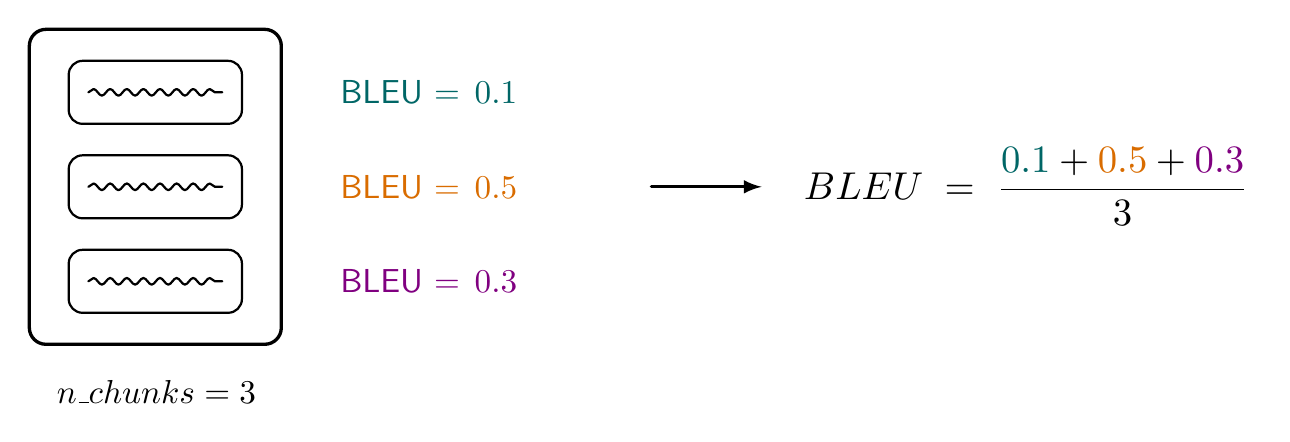
\begin{tikzpicture}[line join=round,line cap=round, >=latex, font=\sffamily]

% --- Left black container with three chunks ---
\draw[black, very thick, rounded corners=6pt]
  (-0.2,3.6) rectangle (3.0,-0.4);

% three inner rounded rectangles
\foreach \y in {2.8,1.6,0.4}{
  \draw[black, thick, rounded corners=5pt] (0.3,\y+0.4) rectangle (2.5,\y-0.4);
  % squiggle inside
  \draw[black, thick, decorate, decoration={snake,amplitude=1.2pt,segment length=6pt}]
    (0.55,\y) -- (2.25,\y);
}

% --- Colored BLEU labels next to each chunk ---
\node[anchor=west, text=teal!80!black, scale=1.2]  at (3.6,2.8) {BLEU $=\,0.1$};
\node[anchor=west, text=orange!85!black, scale=1.2] at (3.6,1.6) {BLEU $=\,0.5$};
\node[anchor=west, text=violet, scale=1.2]         at (3.6,0.4) {BLEU $=\,0.3$};

% --- n_chunks = 3 (black) ---
\node[anchor=west, text=black, scale=1.2] at (0.0,-1.0) {$n\_\text{chunks}=3$};

% --- Arrow to the right and mean BLEU expression ---
\draw[black, very thick, ->, >=latex] (7.7,1.6) -- (9.1,1.6);

\node[anchor=west, text=black, scale=1.4] at (9.3,1.6)
  {$\varnothing\ \text{BLEU} \;=\; \displaystyle
   \frac{\textcolor{teal!80!black}{0.1}+\textcolor{orange!85!black}{0.5}+\textcolor{violet}{0.3}}{3}$};

\end{tikzpicture}
}
  \caption{Computation of the mean BLEU score over 3 text chunks.}
  \label{fig:mean-bleu}
\end{figure}

% Its values range from 0 to 1 \citep{papineni_bleu_2001}.

% \ac{bleu} automatically penalizes n-grams appearing in the candidate text but not in the reference text, 
% as well as n-grams appearing more often in the candidate than in the reference text \citep{papineni_bleu_2001}.

% For multiple sentences, they (1) add the best match (among the reference texts) length for each candidate sentence, 
% and (2) divide this sum $r$ by the total length of all candidate sentences $c$. 
% They cannot use recall for length-related problems here, 
% because \ac{bleu} uses multiple reference texts, which may have different lengths \citep{papineni_bleu_2001,banerjee_METEOR_2005}.
% If the generated candidate is significantly shorter than the reference text, the brevity penalty $BP$ is applied.
% A \ac{bleu} score approaching 1 signifies the candidate matches one reference almost exactly \citep{papineni_bleu_2001}, 
% and thus, limited syntactic diversity (i.e. inadequate paraphrase) \citep{kurt_pehlivanoglu_comparative_2024}.
% Note that more reference texts lead to higher \ac{bleu} scores \citep{papineni_bleu_2001}.

\ac{rouge} \citep{lin_rouge_2004}, initially developed for summarization, is recall-oriented and emphasizes coverage of reference content in the candidate text. 
Several variants exist, including \ac{rouge}-N, which computes n-gram recall, \ac{rouge}-L, which measures the longest common subsequence, and \ac{rouge}-S, which evaluates skip-bigram co-occurrences~\citep{zhou_paraphrase_2021,palivela_optimization_2021,kurt_pehlivanoglu_comparative_2024}. 
\ac{rouge}-L for a candidate $Y$ of length $n$ and a reference $X$ of length $m$, for example, is defined in \autoref{eq:rouge_l}.
For \ac{rouge}-L, the intuition is that the longer the longest common subsequence (LCS) between the candidate and reference texts, the more similar they are \citep{lin_rouge_2004}.
% \ac{rouge}-L requires in-sequence matches that reflect the sentence level word order as n-grams.
% Moreover, no predefined $n$ is necessary, because \ac{rouge}-L includes the longest in-sequence common n-grams.
% However, \ac{rouge}-L does not include shorter sequences or alternative LCSes in the final score~\citep{lin_rouge_2004}.

\begin{equation}
ROUGE-L = F_{lcs} = \frac{(1 + \beta^2)R_{lcs}P_{lcs}}{R_{lcs} + \beta^2 P_{lcs}},
\label{eq:rouge_l}
\end{equation}

$R_{lcs} = \frac{LCS(X,Y)}{m}$ and $P_{lcs} = \frac{LCS(X,Y)}{n}$ capture recall and precision based on subsequence length. 
Although \ac{rouge} is sensitive to word order, it remains a syntactic metric. 
Its ability to reflect semantic adequacy or fluency is limited, and low \ac{rouge} scores may simply reflect lexical diversity rather than paraphrase inaccuracy \citep{kurt_pehlivanoglu_comparative_2024}.

% Its values range from 0 to 1 \citep{kurt_pehlivanoglu_comparative_2024}.
% ROUGE-N
\ac{rouge}-N is an n-gram recall between the candidate text and the reference texts \citep{lin_rouge_2004} as displayed in \autoref{eq:rouge_n}.
\begin{equation}
    ROUGE-N = \frac{\sum_{\mathcal{S} \in \left\{ References \right\}}\sum_{n-gram \in\mathcal{S}}Count_{match}(n-gram)}{\sum_{\mathcal{S'} \in \left\{ References \right\}}\sum_{n-gram' \in\mathcal{S'}}Count(n-gram')}
\label{eq:rouge_n}
\end{equation}
$Count_{match}(n-gram)$ is the maximum number of n-grams co-occuring in the candidate text and the set of reference texts \citep{lin_rouge_2004}.
The nominator sums over all references and thus, gives more weight to matching n-grams that occur in multiple references (i.e. a consensus between references) \citep{lin_rouge_2004}.

% ROUGE-S
A skip-bigram is any pair of words in their sentence order, allowing for arbitrary gaps \citep{lin_rouge_2004}.
\ac{rouge}-S measures the overlap of skip-bigrams between the candidate text and the reference texts \citep{lin_rouge_2004}.
Hence, if the candidate text is the reverse of the reference text, the \ac{rouge}-S score is 0 even though it is not as bad as completely unrelated candidates \citep{lin_rouge_2004}.
\ac{rouge}-SU extends \ac{rouge}-S with unigrams to solve this issue \citep{lin_rouge_2004}.
% ROUGE generally
% \citet{kurt_pehlivanoglu_comparative_2024} claim that \ac{rouge} may not be adequate to assess semantic similarity and fluency.
Lower \ac{rouge} scores indicate greater diversity \citep{kurt_pehlivanoglu_comparative_2024}.

METEOR was proposed to address BLEU's deficiencies. 
Unlike BLEU, which is precision-oriented, METEOR explicitly incorporates recall.
We consider METEOR a syntactic metric due to its conceptual similarity to BLEU, but it captures also semantic characteristics on account of inclusion of stemming and synonym matching modules~\citep{kurt_pehlivanoglu_comparative_2024}. 
Candidate and reference unigrams are first aligned based on modules (exact match, Porter stemmed match, synonymy), after which the best largest subset of unigram mappings is selected according to cardinality and minimal crossing. 
From this alignment, METEOR computes the weighted $F$-score from \autoref{eq:meteor}~\citep{banerjee_METEOR_2005}.

\begin{equation}
    METEOR = F_{mean} = \frac{10 \cdot P \cdot R}{R + 9P} \cdot (1 - Penalty)
\label{eq:meteor}
\end{equation}

The penalty function discourages fragmented matches and reduces the score to $50\%$ bigram or longer matches are absent~\citep{banerjee_METEOR_2005}. 
METEOR has been shown to correlate more strongly with human judgments than BLEU, particularly at the sentence or segment level, due to its sensitivity to lexical and semantic variation \citep{zhou_paraphrase_2021,kurt_pehlivanoglu_comparative_2024}.
% Its values range from 0 to 1 \citep{kurt_pehlivanoglu_comparative_2024}.
$P$ and $R$ denote unigram-precision and unigram-recall respectively~\citep{kurt_pehlivanoglu_comparative_2024,banerjee_METEOR_2005}.
The penality function whenever an incorrect word is encountered~\citep{palivela_optimization_2021} as displayed in \autoref{eq:meteor}.


\subsubsection{Semantic Measures}
Syntactic measures are inadequate when the goal is to evaluate paraphrases that prioritize semantic preservation over lexical similarity. 
To address this limitation, semantic metrics leverage distributed representations of words or sentences.

BERTScore \citep{hanna_fine_grained_2021} computes similarity between contextual BERT embeddings of candidate and reference texts~\citep{hanna_fine_grained_2021}. 
For reference vectors $z$ and candidate vectors $\hat{z}$, precision and recall are defined as \autoref{eq:bert_p} and \autoref{eq:bert_r}, respectively.

\begin{equation}
    P_{BERT} = \frac{1}{|\hat{z}|} \sum_{\hat{z}_j \in \hat{z}} \max_{z_j \in z} z_i\top \hat{z}_j
\label{eq:bert_p}
\end{equation}
\begin{equation}
    R_{BERT} = \frac{1}{|z|} \sum_{z_j \in z} \max_{\hat{z}_j \in \hat{z}} z_i\top \hat{z}_j
\label{eq:bert_r}
\end{equation}

% \begin{equation}
%     F_1 = \frac{2 P_{BERT} R_{BERT}}{P_{BERT} + R_{BERT}} 
% \label{eq:bert_f1}
% \end{equation}
% Since $F_1 \in \left[-1,1\right]$ it can be rescaled to $[0,1]$ by modifying the precision and recall calculation 
% to $\hat{P}_{BERT} = \frac{P_{BERT} - a}{1 - a}$ ($R_{BERT}$ analogous), where $a$ is the empirical lower bound on the BERTScore \citep{hanna_fine_grained_2021}.


BERTScore correlates with human judgment at the semantic level \citep{kurt_pehlivanoglu_comparative_2024}, although it may struggle when lexically overlapping but semantically incorrect candidates are present \citep{hanna_fine_grained_2021}.

\ac{wmd} measures the minimal transport cost of aligning word embeddings from one text to another \citep{gohsen_captions_2023}. 
